\subsubsection{Difusi�n}
\begin{frame}
\frametitle{Difusi�n}

\begin{figure}
\begin{tikzpicture}[node distance=0.5cm, auto,>=latex', thick]
\scriptsize
    % We need to set at bounding box first. Otherwise the diagram
    % will change position for each frame.
    \path[use as bounding box] (-1.5,0) rectangle (12,-2);

    % TT methodology     
    \node [phase]                        (monitoreo)     {Vigilancia};
    \node [phase, below of=monitoreo]    (choice)        {Elecci�n};
    \node [phase, below of=choice]       (acquisition)   {Adquisici�n};
    \node [phase, below of=acquisition]  (adaptation)    {Adaptaci�n};
    \node [phase, below of=adaptation]   (absortion)     {Absorci�n};
    \node [phase, below of=absortion]    (aplication)    {Aplicaci�n};
    \node [phase2,below of=aplication]   (difusion)      {Difusi�n};

    %%%%%%%%%%%%%%%%%%%%%%%%%%%%%%%%%%%%%%%%%%%%&
    %            Difusi�n
    %%%%%%%%%%%%%%%%%%%%%%%%%%%%%%%%%%%%%%%%%%%%&


    \onslide<1> \node [difusion_es, right=1cm of absortion.east] (est_difusion)      
      {
       \begin{center} \textbf{El conocimiento como bien p�blico \cite{CMS06}} \end{center}
       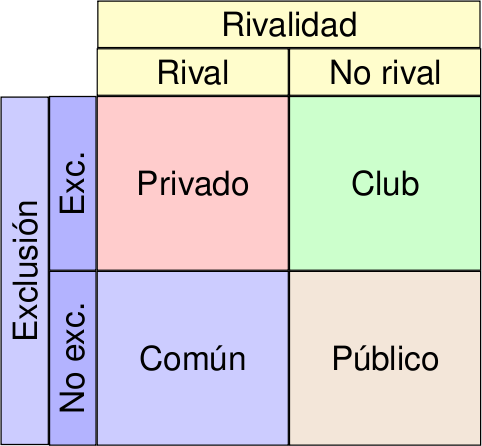
\includegraphics[scale=.4]{../images/bienes_clasific.png}\\
      \begin{center} Ecuaci�n costo-beneficio de Ostrom: \textbf{BC > BN + C\footnote{BC: Beneficio al Contribuir, BN: Costo de no contribuir, C: Costo de la contribuci�n}}\end{center}
      };


%     \onslide<2> \node [difusion_es, right=.5cm of absortion.east] (est_difusion)      
%       {
%        \begin{center} \textbf{Marco para analizar el conocimiento como bien p�blico aplicado a la metodolog�a propuesta} \end{center}
%        \begin{center} 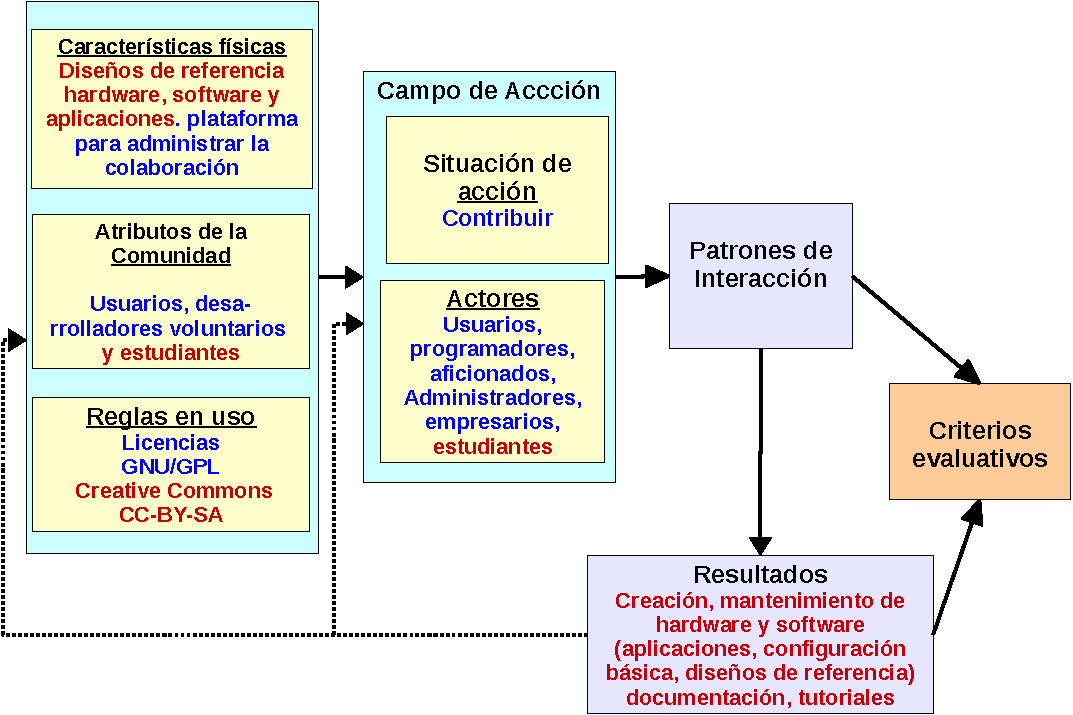
\includegraphics[scale=.47]{../images/framework_hwcl.pdf} \end{center}
%        \begin{center} Ecuaci�n costo-beneficio de Ostrom: \textbf{BC > BN + C\footnote{BC: Beneficio al Contribuir, BN: Costo de no contribuir, C: Costo de la contribuci�n}}\end{center}
%       };



%     \onslide<2> \node [difusion_es, right=1cm of absortion.east] (est_difusion)      
%       {
%        \begin{center} \textbf{Hardware Copyleft vs. Software Libre} \end{center}
%           \setlength\minrowclearance{1pt}
%           \setlength\arrayrulewidth{1pt}
%           \begin{tabular}{|l|l|l|}
%             \hline
%             \rowcolor[rgb]{0.9,0.9,0.4}
%             \bf Concepto          &\bf Software           & \bf Hardware \\
%             \hline
%             C�digo Fuente         & Programa              & Esquem�tico y Layout \\
%             \rowcolor[rgb]{0.8,1,1}
%             Editor                & Editor de Texto       & Sistema EDA \\
%             Conversi�n            & Compilador, etc.      & Sistema EDA \\
%             \rowcolor[rgb]{0.8,1,1}
%             Prueba                & Ejecuci�n             & Prototipo(s) \\
%             Depuraci�n            & Debugger              & Laboratorio \\
%             \rowcolor[rgb]{0.8,1,1}
%             Reproducci�n          & Descarga              & Producci�n, \\
%             \rowcolor[rgb]{0.8,1,1}
%                                   & (Copia perfecta)      & Pruebas \\
%             Distribuci�n          & Internet              & Env�os, Aduanas \\
%             \hline
%           \end{tabular}
% 
%       };

    \onslide<2> \node [ph_explain2, right=.5cm of absortion.east] (est_difusion)      
      {
       \begin{center} \textbf{Hardware Copyleft: Las cuatro libertades $[1]$} \end{center}

          \begin{enumerate}
            \item[0] Ejecutar el programa
              \begin{itemize}
                \scriptsize
                \item Usar el hardware
              \end{itemize}
            \item[1] Estudiar el c�digo
              \begin{itemize}
                \scriptsize
                \item Estudiar los archivos de dise�o (Esquem�tico y layout)
              \end{itemize}
            \item[1] Adaptar el c�digo fuente
              \begin{itemize}
                \scriptsize
                \item Adaptar los archivos de dise�o
                \item Tener acceso a las herramientas para hacerlo
              \end{itemize}
            \item[2,3] Redistribuir copias/modificaciones
              \begin{itemize}
                \scriptsize
                \item Redistribuir los archivos de dise�o
                \item Construir o producir el hardware
              \end{itemize}
          \end{enumerate}

          {\scriptsize $[1]$~\url{http://www.gnu.org/philosophy/free-sw.html}}

      };

%     \onslide<4> \node [ph_explain2, right=.5cm of absortion.east] (est_difusion)      
%       {
%        \begin{center} \textbf{Hardware Copyleft: Requerimientos} \end{center}
%        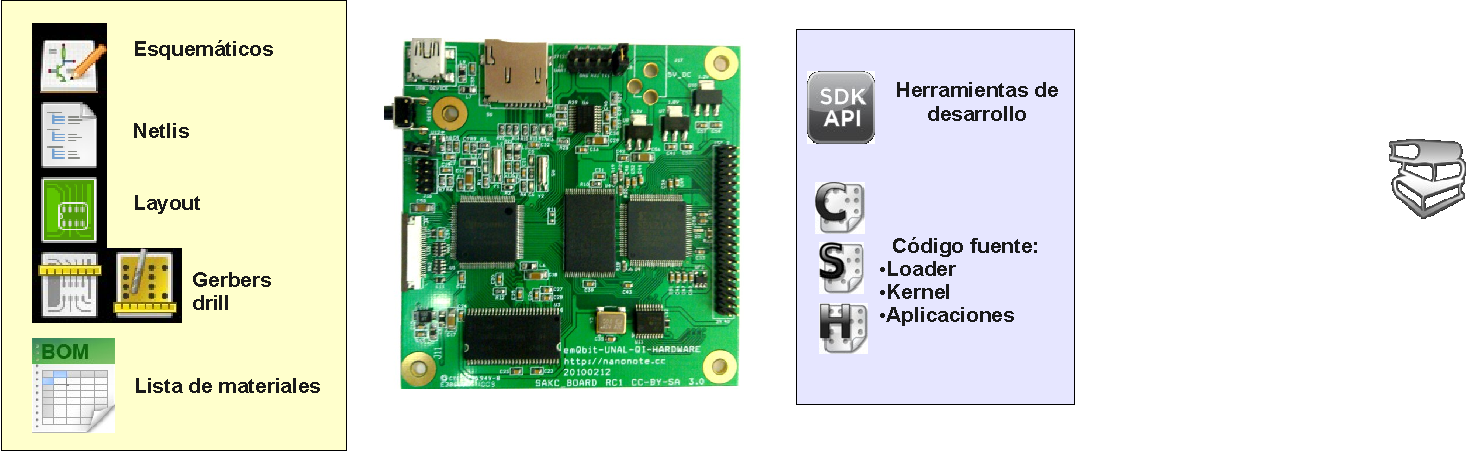
\includegraphics[scale=.5]{../images/copy_left_hardware_requirement.pdf}\\
% %        {\scriptsize Fuente: Werner Almesberger  FISL 12, Brazil}
%       };

    \onslide<3> \node [ph_explain2, right=.1cm of absortion.east] (est_difusion)      
      {
       \begin{center} \textbf{Flujo de dise�o utilizando hardware copyleft} \end{center}
       \begin{center} 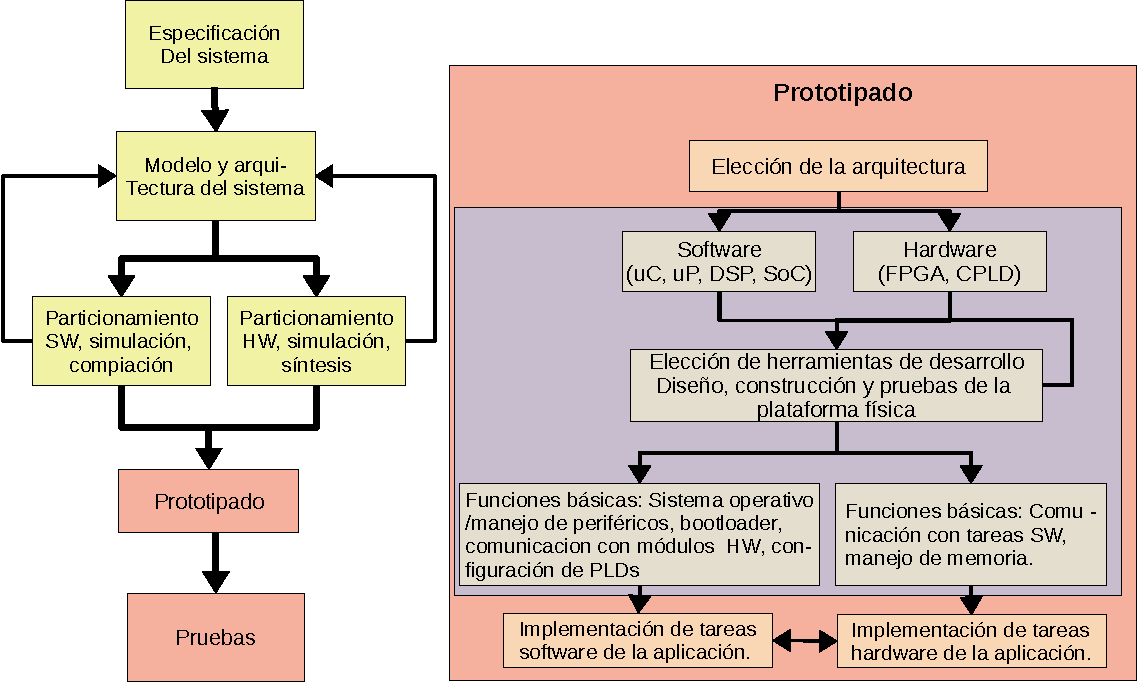
\includegraphics[scale=.48]{../images/design_flow_copyleft_hw.pdf} \end{center}
      };


    %%%%%%%%%%%%%%%%%%%%%%%%%%%%%%%%%%%%%%%%%%%%&
    %        Estrategias de difusi�n
    %%%%%%%%%%%%%%%%%%%%%%%%%%%%%%%%%%%%%%%%%%%%&
    \onslide<4>
      \node [difusion_es, above right=1cm of acquisition.east] (est_difusion)      
      {
       \begin{center} \textbf{Linuxencaja: Estrategia de Difusi�n} \end{center}
       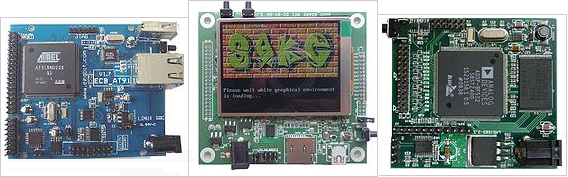
\includegraphics[scale=.25]{../images/plataformas_hwcl.png}\\
       \color{blue!40!black} {Repositorios + Tutoriales + Cursos en l�nea}\\
       \color{green!60!black}{C�digo fuente (.c,.v,.vhd,.S,.java), archivos de dise�o} 

      };

     \node [difusion_es, below = 0.25cm of est_difusion] (canales_difusion)      
      {
       \color{red!60!black} {Canales de difusi�n} \\
                          GIT, WIKI, MAIL
      };

     \draw[myarrow] (est_difusion.south) -- (canales_difusion.north);   



     \node [difusion_es, below = 0.25cm of canales_difusion] (miembros)      
      {
       \begin{center} 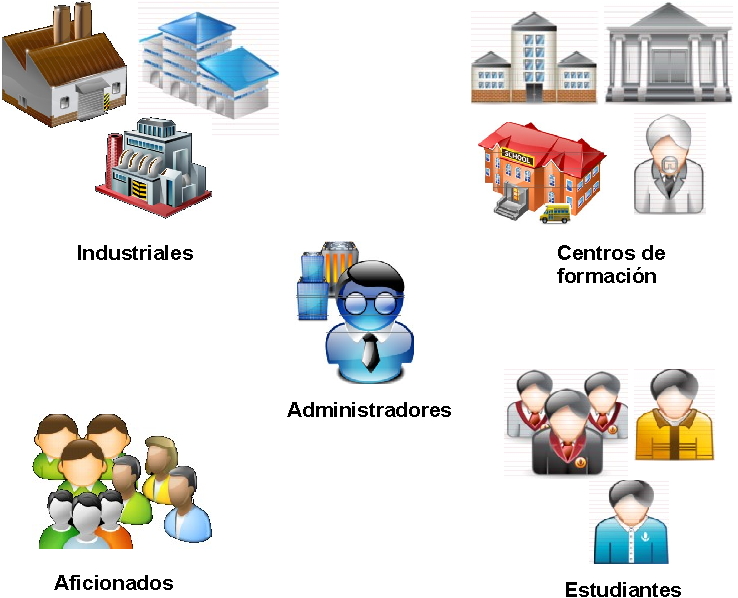
\includegraphics[scale=.4]{../images/community_members.pdf} \end{center}

      };

        \draw[myarrow] (canales_difusion.south) -- (miembros.north);   

    
%      \node [phase2, below = .6cm of canales_difusion] (dif_academia2)      
%       {
%         Academia \\
%         \begin{itemize}
%          \scriptsize
%          \item UIS, ULA, USTA, UDFJC, ENAP.
%          \item ET-ITC.
%          \item SEB.
%         \end{itemize}
%       };
%      \draw[myarrow] (canales_difusion.south) -- (dif_academia2.north);	
%      \node [phase2, left = .1cm of dif_academia2] (dif_academia)      
%       {
%         I+D UNAL \\
%         \begin{itemize}
%          \scriptsize
%          \item Medicina
%          \item Veterinaria
%          \item Mecatr�nica
%          \item Sistemas
%         \end{itemize}
%       };
%      \draw[myarrow] (canales_difusion.south) --++(0,-0.2)--++ (-2.3cm, 0) -- (dif_academia.north);	
%      \node [phase2, right = .1cm of dif_academia2] (dif_industria)      
%       {
%         Industria\\
%          \scriptsize
%         \begin{itemize}
%          \item emQbit.
%          \item $\mu$Ensamble.
%         \end{itemize}
%       };
%      \draw[myarrow] (canales_difusion.south) --++(0,-0.2)--++ (2.3cm, 0) -- (dif_industria.north);
\end{tikzpicture}
\end{figure}

\end{frame}